\chapter{MFCC dan Neutral Network}
Untuk pratikum saat ini menggunakan buku Python Artificial Intelligence Projects for Beginners. Dengan praktek menggunakan python 3 dan editor spyder dan library python keras dan librosa.

\section{Rahmi Roza-1164085}
\subsection{Teori}
\begin{enumerate}
\item Kenapa File Suara Harus Dilakukan MFCC
\begin{itemize}
\item Penjelasan: Agar bisa mengubah suara menjadi vektor. Sehingga data suara bisa diolah menjadi outputan. Jadi semua parameter inputan baik itu suara, dokumen harus dipersiapkan datanya terlebih dahulu, kalau untuk dokumen untuk teks menggunakan word2vec, sedangkan untuk suara menggunakan MFCC (Mel Frequency Cepstral Coeficients) 
\par 
\par
\item Ilustrasi Gambar
\begin{figure}[!hbtp]
\centering
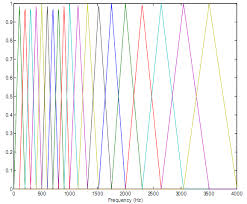
\includegraphics[scale=0.7]{figures/mfccroza.jpg}
\caption{MFCC Roza}
\label{text-fadila}
\end{figure}
\par
\end{itemize}
\par
\par

\item Konsep Dasar Neural Network
\begin{itemize}
\item  Penjelasan:
\par Neural Network merupakan kategori ilmu Soft Computing. Neural Network sebenarnya mengadopsi dari kemampuan otak manusia yang mampu memberikan stimulasi/rangsangan, melakukan proses, dan memberikan output. Output diperoleh dari variasi stimulasi dan proses yang terjadi di dalam otak manusia. Kemampuan manusia dalam memproses informasi merupakan hasil kompleksitas proses di dalam otak. Misalnya, yang terjadi pada anak-anak, mereka mampu belajar untuk melakukan pengenalan meskipun mereka tidak mengetahui algoritma apa yang digunakan.
\par
\item Ilustrasi Gambar
\begin{figure}[!hbtp]
\centering
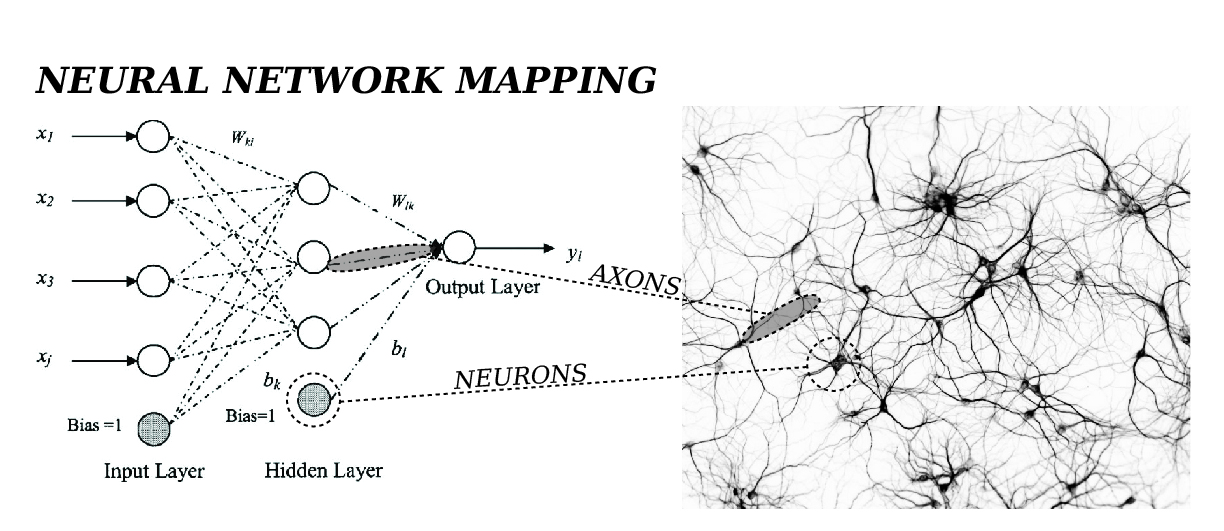
\includegraphics[scale=0.3]{figures/neuralroza.jpg}
\caption{Konsep Dasar Neural Network Roza}
\label{text-fadila}
\end{figure}
\par
\end{itemize}
\par
\par

\item Konsep Pembobotan Dalam Neural Network
\begin{itemize}
\item Penjelasan:
\par Cara kerja Neural Network dapat dianalogikan sebagaimana halnya manusia belajar dengan mengunakan contoh atau yang disebut sebagai supervised learning. Sebuah Neural Network dikonfigurasi untuk aplikasi tertentu, seperti pengenalan pola atau klasifikasi data, dan kemudian disempurnakan melalui proses pembelajaran. Proses belajar yang terjadi dalam sistem biologis melibatkan penyesuaian koneksi sinaptik yang ada antara neuron, dalam halnya pada Neural Network penyesuaian koneksi sinaptik antar neuron dilakukan dengan menyesuaikan nilai bobot yang ada pada tiap konektivitas baik dari input, neuron maupun output.
\par
\item Ilustrasi Gambar
\begin{figure}[!hbtp]
\centering
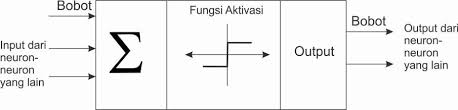
\includegraphics[scale=0.5]{figures/pemboobotanroza.jpg}
\caption{Konsep Pembobotan Roza}
\label{text-fadila}
\end{figure}
\par
\end{itemize}
\par
\par

\item Konsep Fungsi Aktivasi Dalam Neural Network
\begin{itemize}
\item Penjelasan:
\par Setiap neuron mempunyai tingkat aktivasi yang merupakan fungsi dari input yang masuk padanya. Aktivasi yang dikirim suatu neuron ke neuron lain berupa sinyal dan hanya dapat mengirim sekali dalam satu waktu, meskipun sinyal tersebut disebarkan pada beberapa neuron yang lain.
\par
\item Ilustrasi Gambar
\begin{figure}[!hbtp]
\centering
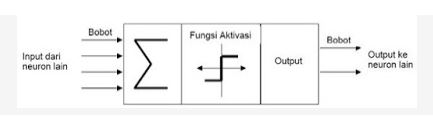
\includegraphics[scale=0.7]{figures/aktivasiroza.jpg}
\caption{Konsep Aktivasi Roza}
\label{text-fadila}
\end{figure}
\par
\end{itemize}
\par
\par

\item Cara Membaca Hasil Plot Dari MFCC
\begin{itemize}
\item Penjelasan:
\par Nanti akan ada outputan berbentuk grafik. Ada 3 dimensi atau sumbu. Dimana untuk sumbu x merupakan waktu, sedangkan sumbu y merupakan frekuensi dari suara yang dihasilkan dalam bentu Hz. Sedangkan pada bagian tengah atau sumbu z merupakan power atau kekuatan dari lagu atau suara atau desibel yang dihasilkan. Untuk melihat penjelasan dari warna pada gambar yang di tengah, maka kita harus mendownload gambar nya terlebih dahuhulu. Untuk warna biru itu merupakan suara rendah, yang merah merupakan tinggi dan daya frekuensi nya berada pada nilai yang rendah karena bass bekerja pada suara yang rendah. Tidak selalu tergantung pada warna untuk menentukan nilai atau frekuensinya. Tetapi pada jenis lagu yang dugunakan. 
\par
\item Ilustrasi Gambar
\begin{figure}[!hbtp]
\centering
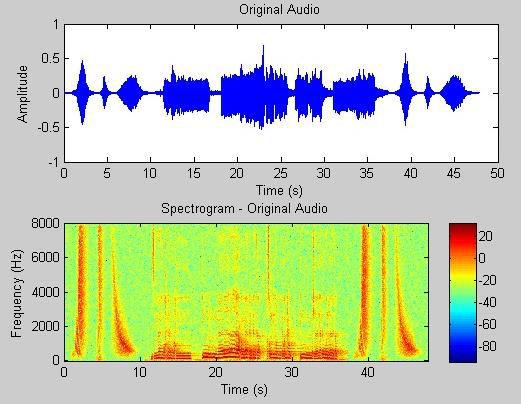
\includegraphics[scale=0.5]{figures/caramembacaroza.jpg}
\caption{Cara Membaca Hasil Plot MLCC Roza}
\label{text-fadila}
\end{figure}
\par
\end{itemize}
\par
\par



\item Apa Itu One-Hot Encoding?
\begin{itemize}
\item Penjelasan:
\par One-hot encoding adalah representasi dari variabel kategori sebagai vektor biner. Yang pertama adalah  mengharuskan nilai kategorikal dipetakan ke nilai integer. Kemudian, setiap nilai integer direpresentasikan sebagai vektor biner yang semuanya bernilai nol kecuali indeks integer, yang ditandai dengan 1.
\par
\item Ilustrasi Gambar
\begin{figure}[!hbtp]
\centering
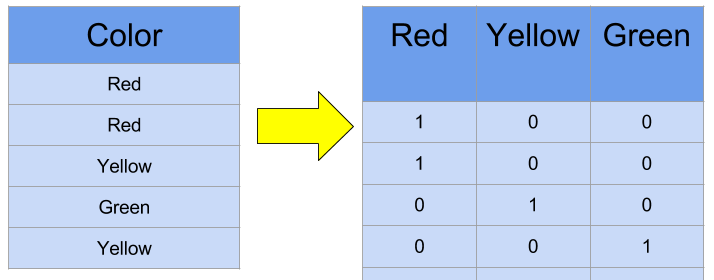
\includegraphics[scale=0.5]{figures/onehotroza.png}
\caption{One Hot Encoding Roza}
\label{bag-fadila}
\end{figure}
\par
\end{itemize}
\par
\par

\item Fungsi Dari np unique dan to categorical dalam kode program
\begin{itemize}
\item  Np.unique
\par 
\item Penjelasan: Untuk mengekstaksi elemen-elemen unik (tertentu) dalam array.
\begin{figure}[!hbtp]
\centering
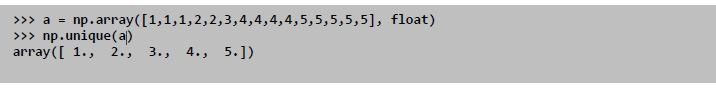
\includegraphics[scale=0.7]{figures/npuniqueroza.jpg}
\caption{NP Unique Roza}
\label{tf-fadila}
\end{figure}
\par
\end{itemize}
\par
\begin{itemize}
\item  To categorical
\par 
\item Penjelasan: Berfungsi untuk mengubah vektor kelas yang berupa integer ( number ) menjadi matriks kelas biner.	
\begin{figure}[!hbtp]
\centering
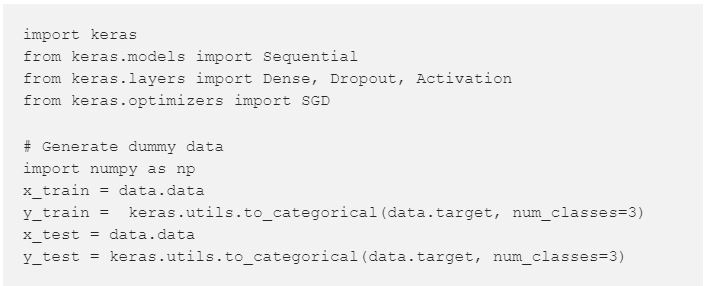
\includegraphics[scale=0.7]{figures/tocategorical.jpg}
\caption{To Categorical roza}
\label{tf-fadila}
\end{figure}
\par
\end{itemize}
\par
\par

\item Fungsi Dari Sequential Pada Kode Program
\begin{itemize}
\item Penjelasan:
\par Sequential proses membandingkan setiap elemen larik satu per satu secara beruntun, mulai dari elemen pertama, sampai dengan elemen terakhir atau elemen yang dicari sudah ditemukan. atau merupakan jenis model yang digunakan dalam perhitungan ataupun code program yang direalisasikan.
\par
\item Ilustrasi Gambar
\begin{figure}[!hbtp]
\centering
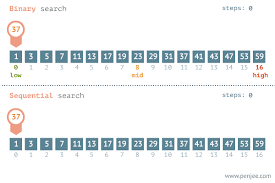
\includegraphics[scale=0.8]{figures/sequentialroza.png}
\caption{Sequential Roza Roza}
\label{text-fadila}
\end{figure}
\par
\end{itemize}
\par
\par

\begin{itemize}
\item Plagiarisme Roza
\begin{figure}[!hbtp]
\centering
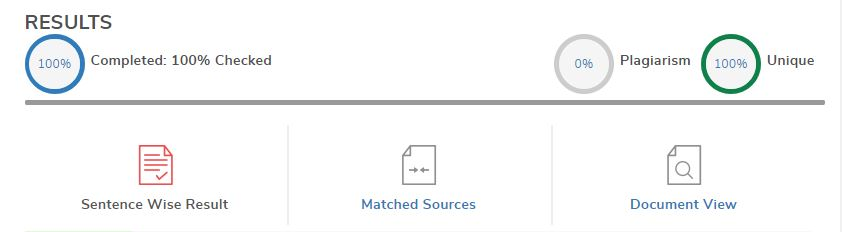
\includegraphics[scale=0.5]{figures/plagiarisme.jpg}
\caption{Plagiarisme Roza}
\label{text-fadila}
\end{figure}
\end{itemize}

\end{enumerate}






\subsection{Praktek}
\begin{enumerate}
\item Menjelaskan Isi Dari Data GTZAN Genre Colection dan Data Freesound
\begin{itemize}
\par Isi dari data GTZAN adalah data musik berdasarkan genre atau jenis dari lagu.Yang sudah di folderkan berdasarkan jenis lagu nya masing-masing.
\lstinputlisting[firstline=8, lastline=20]{src/1164085/1-roza.py}
\par Hasil \ref{no1roza} :
\begin{figure}[!hbtp]
\centering
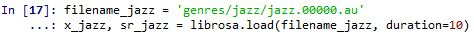
\includegraphics[scale=0.7]{figures/no1roza.jpg}
\caption{Hasil No 1 Roza}
\label{no1roza}
\end{figure}
\par Baris 1: filename jazz merupakan variabel yang berisikan direktori dari file yang dituju, disini digunakan file audio dari genre jazz
\par Baris 2: x jazz dan sr jazz variabel yang digunakan untuk meload file dari variabel filename jazz menggunakan librari Librosa. Yang nantinya akan digunakan pada MFCC
\end{itemize}
\par

\item Menjelaskan Perbaris Kode Fungsi Dari display mfcc()
\begin{itemize}
\item Kode Program
\lstinputlisting[firstline=8, lastline=20]{src/1164085/2-roza.py}
\par Kode Program 2\ref{kpno2} :
\begin{figure}[!hbtp]
\centering
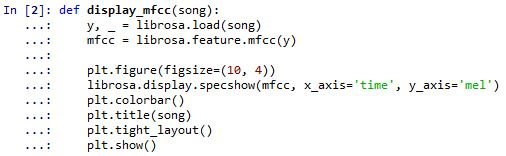
\includegraphics[scale=0.7]{figures/kodeprogram2roza.jpg}
\caption{Kode Program No 2 Roza}
\label{kpno2}
\end{figure}
\end{itemize}
\begin{itemize}
\item Hasil Plot
\par Apabila Sudah Di Plot \ref{hasil2} :
\begin{figure}[!hbtp]
\centering
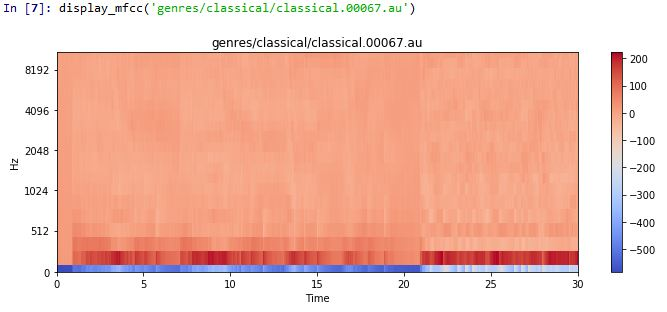
\includegraphics[scale=0.7]{figures/no2roza.jpg}
\caption{Hasil No 2 Roza}
\label{hasil2}
\end{figure}
\par  Baris 1: Membuat fungsi display mfcc untuk menampilkan vektorisasi sebuah suara
\par  Baris 2: Membuat variabel y untuk membaca variabel song dari perintah library load song
\par  Baris 3: Membuat variabel mfcc untuk variabel y dan mengubah suara menjadi vektor
\par  Baris 4: Memplot gambar dengan ukuran 10X4
\par  Baris 5: Menampilkan spektogram atau chromagram agar hasil dari kodingan ini berwarna atau pada grafiknya
\par  Baris 6: Menambahkan colorbar pada plot
\par  Baris 7: Menetapkan judul suara atau lagu
\par  Baris 8: Memberikan label pada sumbu di grafik
\par  Baris 9: Menampilkan hasil plot
\end{itemize}
\par

\item Menjelaskan Kode Program extract features song() dan Mengapa Yang Diambil 25000 Baris Pertama
\begin{itemize}
\item Penjelasan Kode program
\lstinputlisting[firstline=8, lastline=20]{src/1164085/3-roza.py}
\par Hasil 3\ref{hasil3} :
\begin{figure}[!hbtp]
\centering
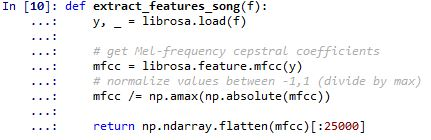
\includegraphics[scale=0.7]{figures/no3roza.jpg}
\caption{Hasil No 3 Roza}
\label{hasil3}
\end{figure}
\par Baris 1: Membuat fungsi extract features song dengan inputan f
\par Baris 2: Membuat variabel y untuk meload inputan f dari perintah librosa load song
\par Baris 3: Membuat variabel mfcc untuk membuat featuredari variabel y
\par Baris 4: Membuat normalisasi nilai antara -1 sampai 1
\par Baris 5: Mengambil 25000 data pertama berdasarkan durasi suara lalu dikembalikan salinan arraynya  dan dikecilkan menjadi satu.
\item Mengapa Yang Diambil 25000 Baris Pertama
\par Diambil 25000 baris pertama karena agar eksekusi data atau saat running tidak memakan waktu yang cukup lama.
\end{itemize}

\item Menjelaskan Kode Program generate features dan labels 
\begin{itemize}
\item Penjelasan Kode program
\lstinputlisting[firstline=8, lastline=20]{src/1164085/4-roza.py}
\par Hasil 4\ref{hasil4} :
\begin{figure}[!hbtp]
\centering
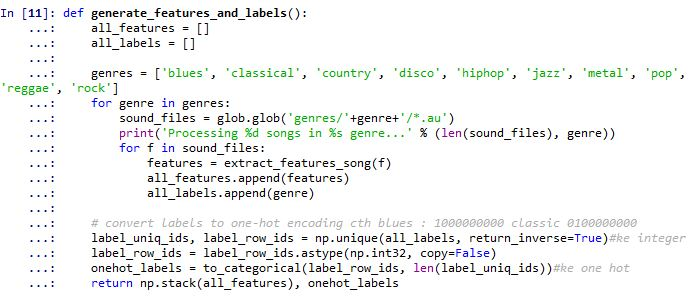
\includegraphics[scale=0.7]{figures/no4roza.jpg}
\caption{Hasil No 4 Roza}
\label{hasil4}
\end{figure}
\par Baris 1: Pembuatan perintah untuk fungi generate geatures dan labels
\par Baris 2: Membuat variabel all features dengan array / parameter kosong
\par Baris 3: Membuat variabel label dengan array / parameter kosong
\par Baris 4: Mendefinisikan variable genres yang didalamnya berisi nama folder-folder pada variabel genres tersebut
\par Baris 5: Membuat perintah looping ( header )
\par Baris 6: Membuat atribut sound files yang berisi perintah looping perfolder dari folder genres dan mengambil semua file berekstensi au ( semuanya dieksekusi berdasarkan module glob ).
\par Baris 7: Menampilkan jumlah song yang dieksekusi.
\par Baris 8: Membuat perintah fungsi dari sound files
\par Baris 9: Membuat variabel features untuk memanggil fungsi extract features song (f) sebagai inputan. Setiap satu file array sound files dilakukan ekstrak fitur.
\par Baris 10: Memasukkan semua features menggunakan perintah append kedalam all features
\par Baris 11: Memasukkan semua genres menggunakan perintah append ke dalam all labels
\par Baris 12: Mendefinisikan label uniq ids dan label row ids sebagai variabel dimana mengeksekusi perintah np.unique dengan parameter variabelnya all labels dan return inverse=True.
\par Baris 13: Membuat variabel label row ids untuk menentukan type dari variabel tersebut dengan type bit yang sesuai dengan yang digunakan.
\par Baris 14: Membuat variabel onehot labels dimana mengeksekusi to categorical dengan variabel parameter low row ids dan len(label uniq ids)
\par Baris 15: Mengembalikan dan menampilkan hasil eksekusi dari variabel parameter all features dan onehot labels perintah dari np.stack.
\end{itemize}
\par


\item Menjelaskan Mengapa Fungsi generate features and labels sangat lama ketika meload dataset genre
\begin{itemize}
\item Kenapa saat load dataset genre lama? karena ada 1000 data yang di proses.
\lstinputlisting[firstline=8, lastline=20]{src/1164085/5-roza.py}
\par Hasil \ref{no5roza} :
\begin{figure}[!hbtp]
\centering
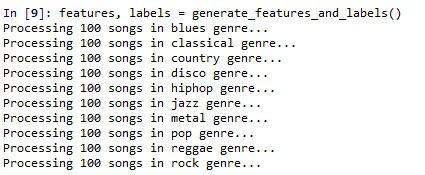
\includegraphics[scale=0.7]{figures/no5roza.jpeg}
\caption{Hasil No 5 Roza}
\label{no5roza}
\end{figure}
\item Penjelasan Hasil:
\par Baris 1: Variabel features and label akn mengeksekusi isi dari features and label
\par Baris 2: Memproses 100 lagu di genre blues
\par Baris 3: Memproses 100 lagu di  genre classical
\par Baris 4: Memproses 100 lagu di  genre country
\par Baris 5: Memproses 100 lagu di  genre disco
\par Baris 6: Memproses 100 lagu di  genre  hip hop
\par Baris 7: Memproses 100 lagu di  genre jazz
\par Baris 8: Memproses 100 lagu di  genre metal
\par Baris 9: Memproses 100 lagu di genre pop
\par Baris 10: Memproses 100 lagu di genre reggae
\par Baris 11: Memproses 100 lagu di genre rock
\end{itemize}
\par

\subsection{Penanganan Error}
\begin{enumerate}
\lstinputlisting[firstline=8, lastline=20]{src/1164085/error-roza.py}
\item Skrinsut Error
\begin{figure}[ht]
\centering
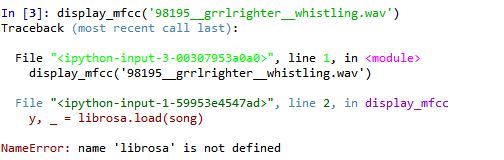
\includegraphics[scale=0.7]{figures/erorroza.jpeg}
\caption{ Error Roza}
\label{6}
\end{figure}
\item Kode Error dan Jenis Errornya
\par Kode Error: "Name Error" name 'librosa' is not defined
\par Jenis Error: Nama Librosa Tidak terdefinisi
\item Penanganan
\par Mendefinisikan library librosa

\end{enumerate}
\end{enumerate}








\par
\par
\section{Fadila-1164072}
\subsection{Teori}
Penjelasan Tugas Harian 11 ( No 1-8 ).
\begin{enumerate}
\item Mengapa File Suara Harus Dilakukan MFCC Dilengkapi Dengan Ilustrasi Atau Gambar :
\par Perlu diketahui terlebih dahulu bahwa MFCC ( Mel Frequency Cepstral Coefficients ) merupakan koefisien yang merepresentasikan audio ( lebih simpelnya digunakan sebagai library ). Ekstraksi ciri dalam proses ini ditandai dengan pengubahan data suara menjadi data citra berupa spektrum gelombang.
\begin{itemize}
\item Penjelasan File Suara Harus Dilakukan MFCC : 
\par Diharuskan melakukan MFCC kepada objek suara agar suara dapat berubah / diubah ke dalam bentuk data matrix dimana telah dilakukan ekstraksi oleh MFCC ( data citra berupa spektrum gelombang ) kemudian direalisasikan sebagai data matrix. Suara tersebut menjadi vektor yang nantinya akan diolah jadi outputan.
\par
\item Ilustrasi Gambar : \ref{suara-mfcc-fadila}
\par
\begin{figure}[!hbtp]
\centering
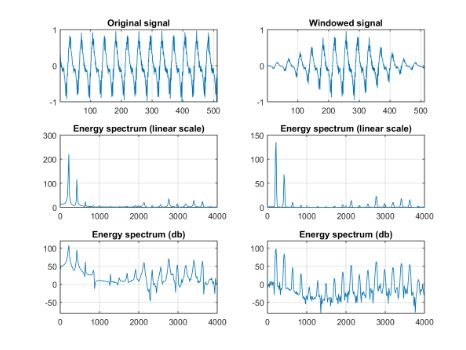
\includegraphics[scale=0.2]{figures/suara-mfcc-fadila.jpg}
\caption{Suara Harus Dilakukan MFCC - fadila}
\label{suara-mfcc-fadila}
\end{figure}
\par
\par Penjelasan :
\par Pada gambar tersebut, digambarkan sebuah bingkai dari klip suara bernyanyi untuk pengujian yang sama. Dengan menggunakan jendela Hamming, harmonik dalam respons frekuensi jauh lebih tajam.Untuk bingkai input terdiri dari 3 periode fundamental yang identik, maka respons frekuensi magnitudo akan dimasukkan 2 nol antara setiap dua titik tetangga dari respons frekuensi dari periode fundamental tunggal. Dengan kata lain, harmonik dari respons frekuensi umumnya disebabkan oleh periode fundamental berulang dalam bingkai. 
\par
\par
\end{itemize}
\par
\par
\item Konsep Dasar Neural Network Dilengkapi Dengan Ilustrasi Atau Gambar :
\par Neural Network merupakan sistem komputasi yang efisien yang tema utamanya dipinjam dari analogi jaringan saraf biologis. JST juga disebut sebagai "sistem saraf tiruan," atau "sistem pemrosesan terdistribusi paralel," atau "sistem koneksionis."
\begin{itemize}
\item Penjelasan Konsep Dasar Neural Network : ( Proses Kerja Saraf Pada Manusia )
\par Ide dasar Neural Network dimulai dari otak manusia atau terkenal yang diawali dengan karya fisiolog, dimana otak memuat sekitar 1011 neuron. Untuk setiap dari sel yang dihasilkan akan saling berinteraksi satu sama lain yang menghasilkan kemampuan tertentu pada kerja otak manusia.
\par
\item Ilustrasi Gambar : \ref{konsep-neu-fadila}.
\par
\begin{figure}[!hbtp]
\centering
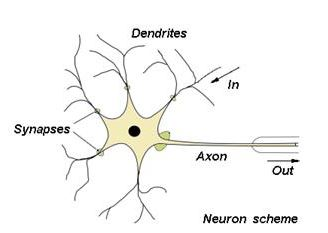
\includegraphics[scale=0.2]{figures/konsep-neu-net-fadila.jpg}
\caption{Konsep Dasar Neural Network- fadila}
\label{konsep-neu-fadila}
\end{figure}
\par
\par Penjelasan :
\par Gambar tersebut mendefinisikan beberapa hal berikut :
\begin{enumerate}
\item Untuk Dendrit (Dendrites) berfungsi untuk mengirimkan impuls yang diterima ke badan sel syaraf.
\item Untuk Akson (Axon) berfungsi untuk mengirimkan impuls dari badan sel ke jaringan lain
\item Untuk Sinapsis berfungsi sebagai unit fungsional di antara dua sel syaraf.
\end{enumerate}
\par Secara keseluruhan dapat dijelaskan bahwa Sebuah neuron menerima impuls dari neuron lain melalui dendrit dan mengirimkan sinyal yang dihasilkan oleh badan sel melalui akson. Akson dari sel syaraf ini bercabang-cabang dan berhubungan dengan dendrit dari sel syaraf lain dengan cara mengirimkan impuls melalui sinapsis.
\par
\end{itemize}
\par
\par
\item Konsep Pembobotan Neural Network Dilengkapi Dengan Ilustrasi Atau Gambar :
\begin{itemize}
\item Penjelasan Konsep Pembobotan Neural Network :
\par  Sebuah Neural Network dikonfigurasi untuk aplikasi tertentu, seperti pengenalan pola atau klasifikasi data. Terjadi penglibatan dalam penyesuaian koneksi sinaptik yang ada antara neuron ketika melakukan penyempurnaan dengan proses pembelajaran. Penyesuaian nilai bobot yang ada pada tiap konektivitas baik dari input, neuron maupun output disinkronkan dengan penyesuaian koneksi sinaptik antar neuron itu sendiri.
\par
\item Ilustrasi Gambar : \ref{bobot-neu-fadila}.
\par
\begin{figure}[!hbtp]
\centering
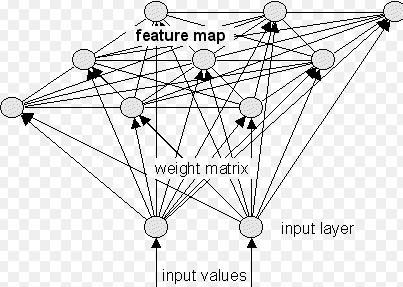
\includegraphics[scale=0.2]{figures/bobot-neu-fadila.jpg}
\caption{Pembobotan Pada Neural Network- fadila}
\label{bobot-neu-fadila}
\end{figure}
\par
\par
\end{itemize}
\par
\par
\item Konsep Fungsi Aktifasi Dalam Neural Network Dilengkapi Dengan Ilustrasi Atau Gambar :
\begin{itemize}
\item Penjelasan Konsep Fungsi Aktifasi Dalam Neural Network :
\par Operasi matematik yang dikenakan pada sinyal output y. Fungsi ini akan digunakan untuk pengaktifan dan juga penonaktifan neuron. Perilaku dari JST ( jaringan saraf tiruan ) ditentukan oleh bobot beserta dengan masukan-keluaran fungsi aktivasi yang ditetapkan.
\item Dalam Konsep Fungsi Aktivasi Neuron Network Terdapat Beberapa Jenis :
\begin{itemize}
\item Fungsi Undak Biner Hard Limit ( Menkonversi nilai masukan dari suatu variabel )
\item Fungsi Undak Biner Threshold ( Menggunakan nilai ambang 0 sebagai batas eksekusil )
\item Fungsi Bipolar Symetric Hard Limit ( Mempunyai keluaran bernilai 1 dan 0 )
\item Fungsi Bipolar Threshold ( Mempunyai keluaran bernilai 1, 0 atau -1 )
\item Fungsi Linear ( Nilai masukan dan keluaran sama )
\item Fungsi Saturating Linear ( Keluarannya bernilai satu apabila masukkanya lebih dari 0 )
\par
\end{itemize}
\item Ilustrasi Gambar : \ref{fungsi-aktivasi-fadila}.
\par
\begin{figure}[!hbtp]
\centering
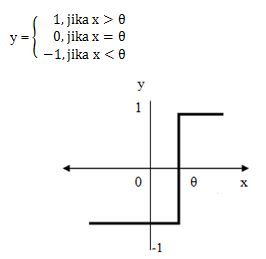
\includegraphics[scale=0.2]{figures/fungsi-aktivasi-fadila.jpg}
\caption{Fungsi Aktifasi - fadila}
\label{fungsi-aktivasi-fadila}
\end{figure}
\par
\par Penjelasan : ( Contoh Fungsi Aktivasi Neural Network : Bipolar Threshold )
\par Pada gambar tersebut menjelaskan bahwa fungsi ini mempunyai keluaran atau outputan yang bernilai 1,0 ataupun -1 untuk batas nilai ambang 0 tertentu. Secara sistematis, fungsi tersebut dapat digambarkan seperti contoh yang telah diberikan.
\par
\par
\end{itemize}
\par
\par
\item Cara Membaca Hasil Plot Dari MFCC Dilengkapi Dengan Ilustrasi Atau Gambar :
\begin{itemize}
\item Pembacaan Hasil Plot Dari MFCC : ( berdasarkan contoh )
\par Untuk hasil ploting dari MFCC, perhitungan pada prosesnya melibatkan atau mendefinisikan pemrosesan sinyal dimana terdapat 430 sampel yang tumpang tindih dengan 215 sampel (kesetaraan jendela ~ 50 ms) kemudian di terapkan jendela Hamming ke sebuah segmen (Hitung FFT: X = fft (x) ). Perhitungan energi tidak termasuk pada bagian frekuensi negatif oleh karena hanya diambil frekuensi antara 0-4kHz. Kemudian di dapatlah bank 40 filter berbentuk segitiga dengan pusat tersebar di frekuensi mel antara 20Hz dan 4kHz.
\par
\item Ilustrasi Gambar : \ref{hasil-plot-1-fadila} dan \ref{hasil-plot-2-fadila}.
\par
\begin{figure}[!hbtp]
\centering
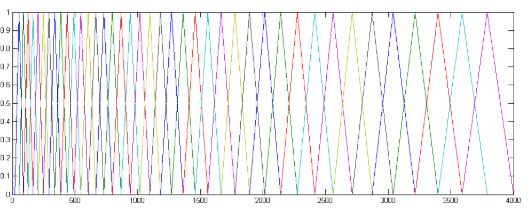
\includegraphics[scale=0.2]{figures/hasil-plot-1-fadila.jpg}
\caption{Pembacaan Hasil Plot MFCC- fadila}
\label{hasil-plot-1-fadila}
\end{figure}
\par
\begin{figure}[!hbtp]
\centering
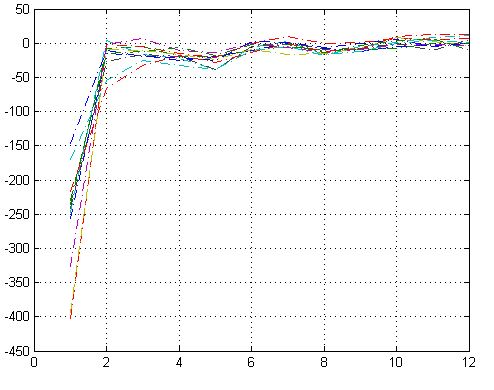
\includegraphics[scale=0.2]{figures/hasil-plot-2-fadila.jpg}
\caption{Pembacaan Hasil Plot MFCC- fadila}
\label{hasil-plot-2-fadila}
\end{figure}
\end{itemize}
\par
\par
\item Apa itu One-Hot Encoding Dilengkapi Dengan Ilustrasi Atau Gambar :
\begin{itemize}
\item Penjelasan One-Hot Encoding : 
\par Proses di mana variabel kategorikal dikonversi menjadi bentuk yang dapat disediakan untuk algoritma ML untuk melakukan pekerjaan yang lebih baik dalam prediksi.
\par
\par
\item Ilustrasi Code Dan Gambar :
\begin{enumerate}
\item Ilustrasi 1 : \ref{one-hot-en-fadila} dan \ref{one-hot-en-2-fadila}.
\par
\begin{figure}[!hbtp]
\centering
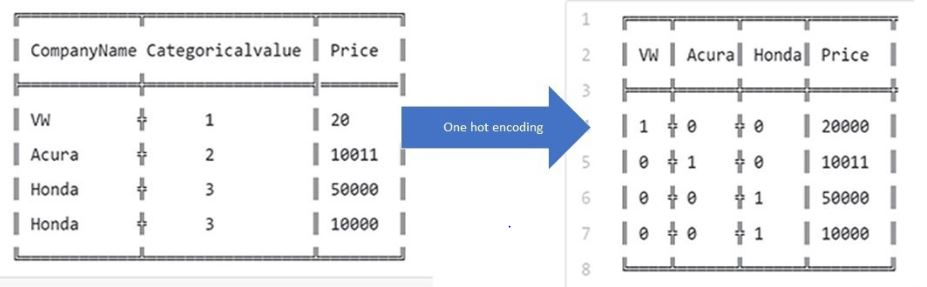
\includegraphics[scale=0.2]{figures/one-hot-en-fadila.jpg}
\caption{One-Hot Encoding 1- fadila}
\label{one-hot-en-fadila}
\end{figure}
\par
\begin{figure}[!hbtp]
\centering
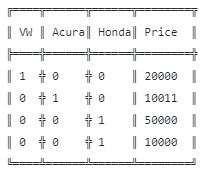
\includegraphics[scale=0.2]{figures/one-hot-en-2-fadila.jpg}
\caption{One-Hot Encoding 1- fadila}
\label{one-hot-en-2-fadila}
\end{figure}
\par
\par Penjelasan :
\par Nilai kategoris mewakili nilai numerik dari entri dalam dataset. Dicontohkan apabila ada perusahaan lain dalam dataset, itu akan diberi nilai kategoris sebagai 4. Ketika jumlah entri unik meningkat, nilai kategoris juga meningkat secara proporsional. Tabel sebelumnya hanyalah representasi. Pada kenyataannya, nilai-nilai kategorikal mulai dari 0 sampai dengan kategori N-1. 
\par Inimerupakan bentuk organisasi yang didefinisikan dengan VW> Acura> Honda berdasarkan pada nilai-nilai kategorikal. Rata-rata VW dan Honda adalah Acura, dengan menggunakan satu one-hot encoding untuk melakukan "binarisasi" kategori dan memasukkannya sebagai fitur untuk melatih model sehingga memberikan hasil yang sesuai.
\par
\item Ilustrasi 2 : \ref{one-hot-en-3-fadila}.
\begin{lstlisting}
from numpy import array
from numpy import argmax
from keras.utils import to_categorical
# define example
data = [1, 3, 2, 0, 3, 2, 2, 1, 0, 1]
data = array(data)
print(data)
# one hot encode
encoded = to_categorical(data)
print(encoded)
# invert encoding
inverted = argmax(encoded[0])
print(inverted)
\end{lstlisting}
\par
\begin{figure}[!hbtp]
\centering
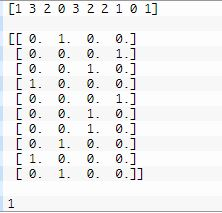
\includegraphics[scale=0.2]{figures/one-hot-en-3-fadila.jpg}
\caption{One-Hot Encoding 2 - fadila}
\label{one-hot-en-3-fadila}
\end{figure}
\par
\par Penjelasan :
\par Pada gambar tersebut dijelaskan bahwa terdapat bilangan bulat yang kemudian dikodekan sebagai vektor biner dan dicetak. Kemudian dapat dilihat bahwa nilai integer pertama 1 dikodekan sebagai [0, 1, 0, 0].Selanjutnya membalikkan pengkodean dengan menggunakan fungsi argumax NumPy () pada nilai pertama dalam urutan yang mengembalikan nilai yang diharapkan 1 untuk bilangan bulat pertama.
\end{enumerate}
\end{itemize}
\par
\par
\item Fungsi Dari Unp.Unique Beserta To.Categorical Dilengkapi Dengan Ilustrasi Atau Gambar :
\begin{enumerate}
\item Penjelasan Fungsi Dari Unp.Unique :
\par Berfungsi untuk menemukan elemen unik array. Dimana dapat , mengembalikan elemen unik array yang diurutkan. Ada tiga output opsional selain elemen unik :
\begin{itemize}
\item indeks array input yang memberikan nilai unik
\item indeks array unik yang merekonstruksi array input
\item berapa kali setiap nilai unik muncul dalam array input
\end{itemize}
\par
\par Ilustrasi Gambar : \ref{np-unique-fadila}.
\par
\begin{figure}[!hbtp]
\centering
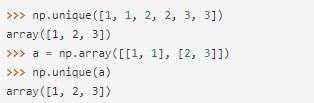
\includegraphics[scale=0.2]{figures/np-unique-fadila.jpg}
\caption{Np.Unique - fadila}
\label{np-unique-fadila}
\end{figure}
\par
\par Penjelasan :
\par Pada gambar tersebut, secara garis besarnya np.unique mengambil data yang berbeda dari variabel a yang berada dalam array modul np itu sendiri. Pada contoh terdapat nilai 1 yang memiliki pengulangan angka, maka hanya salah satu diantara angka tersebut yang ditampilkan bukan keduanya yang diikuti dengan angka berbeda lainnya. Hasilnya yang telah digambarkan pada contoh.
\par
\par
\item Penjelasan Fungsi Dari To\_Categorical :
\par Berfungsi untuk mengubah vektor kelas yang berupa integer ( number ) menjadi matriks kelas biner.
\par
\begin{itemize}
\item Ilustrasi Gambar : \ref{to-categorical-fadila}.
\par
\begin{figure}[!hbtp]
\centering
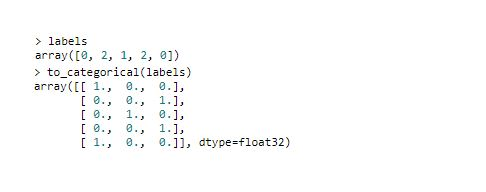
\includegraphics[scale=0.2]{figures/to-categorical-fadila.jpg}
\caption{To Categorical - fadila}
\label{to-categorical-fadila}
\end{figure}
\par
\par
\par Penjelasan :
\par Pada gambar berikut di contoh penerapan array dari 5 label yang telah diset mejadi 3 kelas. Kemudian to\_categorical difungsikan untuk mengkonversi array tersebut kedalam matrix sebanyak dari kolom-kolom yang ada pada kelas tersebut. Jumlah dari barisnya akan tetap sama dengan yang telah dieksekusi sebelumnya. Dan jadilah hasil seperti contoh tersebut.
\par
\par
\end{itemize}
\end{enumerate}
\par
\par
\item Fungsi Dari Sequential Dilengkapi Dengan Ilustrasi Atau Gambar :
\begin{itemize}
\item Penjelasan Fungsi Dari Sequential :
\par Sebuah jenis model yang digunakan dalam perhitungan ataupun code program yang direalisasikan. Neural Networks Sequential membangun fitur tingkat tinggi melalui lapisannya yang berurutan. Sequential juga merupakan proses dimana membandingkan setiap elemen larik satu per satu secara beruntun, mulai dari elemen pertama, sampai dengan elemen terakhir atau elemen yang dicari sudah ditemukan.
\par
\item Ilustrasi Gambar : \ref{sequential-fadila}.
\par
\begin{figure}[!hbtp]
\centering
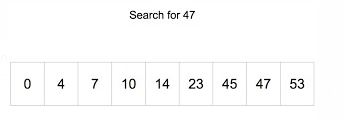
\includegraphics[scale=0.2]{figures/sequential-fadila.jpg}
\caption{Sequential - fadila}
\label{sequential-fadila}
\end{figure}
\par
\par Penjelasan :
\par Pada gambar diatas, mendefinisikan pencarian terhadap angka 47 dimana hasilnya tetap diurutkan sesuai dengan elemennya.
\par
\par
\end{itemize}
\par
\par
\item Plagiarism :
\par
\begin{figure}[!hbtp]
\centering
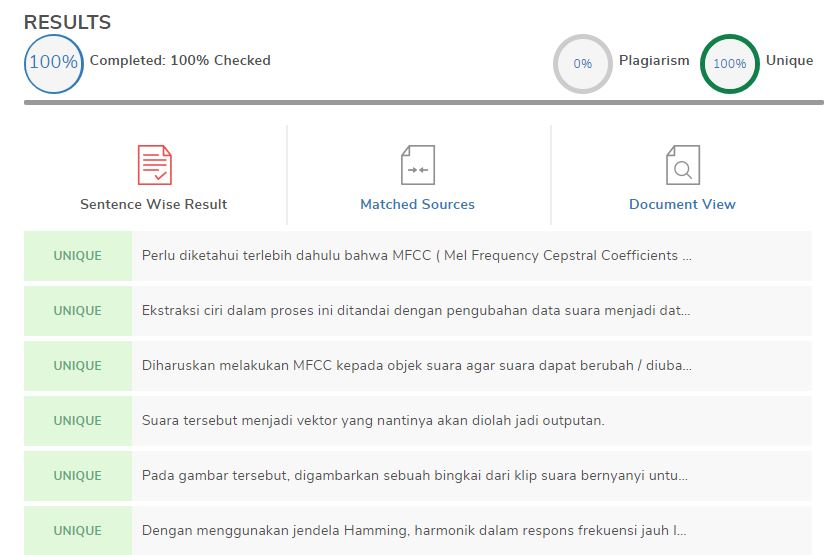
\includegraphics[scale=0.3]{figures/plagiarismmmm-fadila.jpg}
\caption{Plagiarisme- fadila}
\label{plagiarisme-fadila}
\end{figure}
\par
\end{enumerate}

\section{Lusia Violita Aprilian-1164080}

\subsection{Teori}

\begin{enumerate}
\item Jelaskan kenapa file suara harus di lakukan MFCC.
	\begin{itemize}
	\item Jawaban :
		\par MFCC (Mel Frequency Cepstral Coeficients) digunakan untuk mengubah file suara kedalam bentuk vektor. Dan mengapa harus dilakukan MFCC? Jawabannya ialah supaya file suara tersebut dapat diolah kembali menjadi output-an. Dan semua parameter inputan baik itu suara maupun dokumen harus dipersiapkan datanya terlebih dahulu. 
	\item Ilustrasi Gambar :
		\par Berikut adalah ilustrasi penggambaran dari MFCC :
		\begin{figure}[!hbtp]
		\centering
		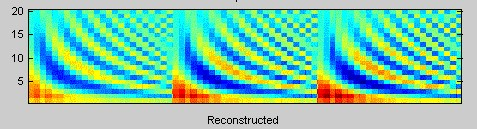
\includegraphics[scale=0.4]{figures/s1.jpg}
		\caption{Lusia-MFCC}
		\label{6A1}
		\end{figure}
	\end{itemize}
	
\item Jelaskan konsep dasar neural network.
	\begin{itemize}
	\item Jawaban :
		\par Konsep dasar yang digunakan pada nural network mengadopsi mekanisme berfikir dari struktur dan proses kerja neuron pada otak manusia. Dimana otak manusia dapat bekerja untuk memberikan stimulasi atau rangsangan, melakukan proses, dan memberikan output-an. Baik untuk memproses sebagai sinyal elemen yang diterima, toleransi terhadap kesalahan, maupun pada proses paralel.
	\item Ilustrasi Gambar :
		\par Berikut adalah ilustrasi penggambaran pada konsep dasar neural network :
		\begin{figure}[!hbtp]
		\centering
		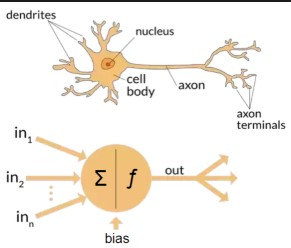
\includegraphics[scale=0.4]{figures/s2.jpg}
		\caption{Lusia-Neural Network}
		\label{6A2}
		\end{figure}
	\end{itemize}
	
\item Jelaskan konsep pembobotan dalam neural network.
	\begin{enumerate}
	\item Jawaban :
		\par Bobot merupakan jembatan yang menghubungkan neuron satu dengan neuron yang lainnya. Dimana pada proses neural network dimulai dari input yang diterima neuron beserta nilai bobot. Nilai bobot tersebut sebagai penanda dari sebuah koneksivitas. Selanjutnya nilai inputan akan dihitung dan menghasilkan aktif atau tidak. Apabila data aktif, neuron mengirimkan nilai output melalui bobot output-nya ke semua neutron yang terhubung. 
	\item Ilustrasi Gambar :
		\par Berikut adalah ilustrasi penggambaran pada konsep pembobotan :
		\begin{figure}[!hbtp]
		\centering
		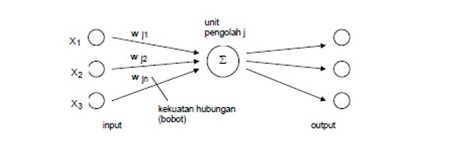
\includegraphics[scale=0.4]{figures/s3.jpg}
		\caption{Lusia-Konsep Pembobotan}
		\label{6A3}
		\end{figure}
	\end{enumerate}
	
\item Jelaskan konsep fungsi aktivasi dalam neural network. 
	\begin{itemize}
	\item Jawaban :
		\par Fungsi aktivasi pada neural network berfungsi layaknya sinapsis pada neuron manusia. Dimana pada neural network, fungsi aktivasi sebagai penentu aktivasi dari sebuah nilai input-an yang sebelumnya telah dihitung pada hidden layer.
	\item Ilustrasi gambar :
		\par Berikut adalah ilustrasi penggambaran pada konsep fungsi aktivasi :
		\begin{figure}[!hbtp]
		\centering
		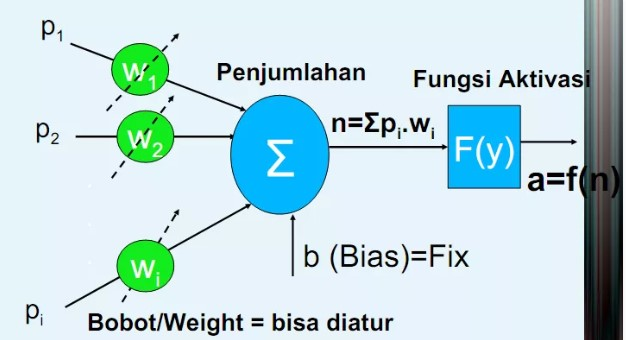
\includegraphics[scale=0.5]{figures/s4.jpg}
		\caption{Lusia-Konsep Fungsi Aktivasi}
		\label{6A4}
		\end{figure}
	\end{itemize}
	
\item Jelaskan cara membaca hasil plot dari MFCC.
	\begin{itemize}
	\item Jawaban :
		\par Pada sebuah grafik hasil plot dari MFCC, terdapat 2 sumbu yaitu x dan y. Sumbu x merupakan waktu atau durasi dari sebuah suara/musik/lagu, sedangkan sumbu y merupakan frekuensi dari suara yang dihasilkan, dan hasilnya merupakan desibel/power. Desibel yang dihasilkan memiliki range warna yang berbeda-beda. Range warna dari desibel adalah mulai dari biru tua hingga coklat tua. Range warna biru merupakan suara yang tidak dapat didengar manusia dan coklat merupakan suara yang dapat dapat didengar manusia.
	\item Ilustrasi gambar :
		\par Berikut adalah ilustrasi dari cara membaca hasil plot dari file whistling.wav :
		\begin{figure}[!hbtp]
		\centering
		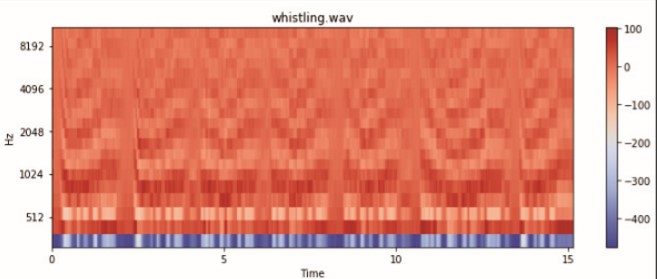
\includegraphics[scale=0.5]{figures/s5.jpg}
		\caption{Lusia-Membaca hasil plot}
		\label{6A5}
		\end{figure}
		
	\end{itemize}
\item Jelaskan apa itu one-hot encoding.
	\begin{itemize}
	\item Jawaban :
		\par one-hot encoding adalah proses di mana variabel kategorikal dikonversi menjadi bentuk yang tersedia pada algoritma Machine Learning (vektor biner) untuk melakukan prediksi. Nilai kategirokal akan dipetakan ke bentuk biner, lalu nilai integer diubah atau dipresentasikan kedalam bentuk vektor biner yang semua nilainya bernilai nol kecuali indeks integer.
	\item Ilustrasi gambar :
		\par Berikut adalah ilustrasi penggambaran one-hot encoding :
		\begin{figure}[!hbtp]
		\centering
		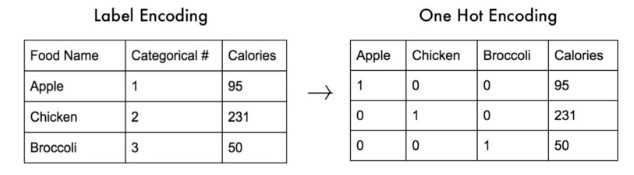
\includegraphics[scale=0.4]{figures/s6.jpg}
		\caption{Lusia-one hot encoding}
		\label{6A6}
		\end{figure}
	\end{itemize}
	
\item Jelaskan apa fungsi dari np.unique dan to\_categorical dalam kode program.
	\begin{itemize}
	\item np.unique 
		\par np.unique atau numpy.unique yang berfungsi untuk menemukan elemen unik pada array.
		\begin{figure}[!hbtp]
		\centering
		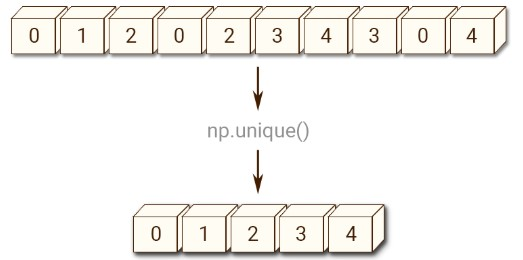
\includegraphics[scale=0.4]{figures/s7a.jpg}
		\caption{Lusia-np.unique}
		\label{6A7}
		\end{figure}
	\item to\_categorical
		\par to\_categorical digunakan untuk meng-convert atau mengubah class vector berupa integer ke dalam matrix kelas biner.
		\begin{figure}[!hbtp]
		\centering
		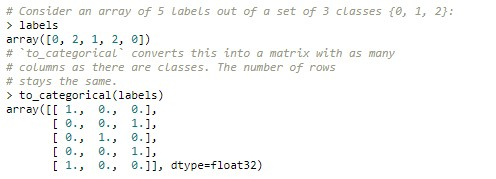
\includegraphics[scale=0.4]{figures/s7b.jpg}
		\caption{Lusia-to categorical}
		\label{6A8}
		\end{figure}
	\end{itemize}
	
\item Jelaskan apa fungsi dari Sequential dalam kode program.
	\begin{itemize}
	\item Jawaban :
		\par Sequential merupakan proses untuk membandingkan setiap satu larik elemen dengan cara satu persatu secara beruntun. Atau pada library keras, sequential merupakan sebuah model.
	\item Ilustrasi gambar :
		\par Berikuta adalah gambaran ilustrasi dari sequential.
		\begin{figure}[!hbtp]
		\centering
		
\includegraphics[scale=0.4]{figures/s8.jpg}
		\caption{Lusia-sequential}
		\label{6A9}
		\end{figure}
	\end{itemize}
\end{enumerate}

\subsection{Praktek}